\section{Processing methods}
Looking at the challenges presented in the previous section it is obvious that there are numerous factors, in which the existing state-of-the-art systems for capacitive sensing can be improved. 
\subsection{Sparsely distributed sensor arrays}
\label{ch:proc_sparse}
Sparsely distributed sensor arrays are layouts that limit the number of available sensors, either by environmental parameters or by design. This limits the information that can be gathered about the detectable object, or reduces the number of different objects that can be distinguished. To compensate this limitation a number of interpolation methods can be used that take into account our knowledge about the position and shape of the electrodes that are used in the current setup. One example for this sparse distribution is the previously presented Thracker system that uses only four electrodes to acquire a hand position and detect gestures at certain positions \cite{Wimmer2007a}. In this section I will present two different contributions - a new method to recognize single-hand gestures in free-air, using just six different sensors, and an indoor localization system based on a coarse grid of wire electrodes that can be hidden below different floor surfaces.

\subsubsection{3D location tracking and gesture interaction}
\begin{figure}[h]
\centering
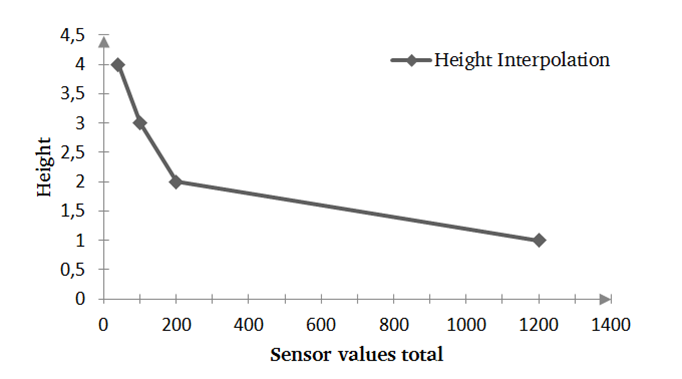
\includegraphics[width=0.6\textwidth]{images/magicbox_data_zaxis}
\caption{Piecewise linear hand distance estimation \cite{Braun2011MultiInputDevice}}
\label{fig:magicbox_data_zaxis}
\end{figure}

Gesture recognition can comprise a large number of different body movements, including sign language that uses movements and position of hands and fingers, the posture of the whole body, or as in our case the movement of the hand in three dimensions. This requires two distinct processing steps. At first it is necessary to precisely localize the position of the hand in the interaction space. Afterwards, a time series of theses positions has to be analyzed and attributed to different gestures. The localization method was first presented in a publication from 2011 \cite{Braun2011MultiInputDevice}. The static gesture recognition method used there was later extended by adapting algorithms used to detect mouse gestures for movements in three dimensions \cite{braun2013capacitive}. 
The first data processing step is the planar localization of the hand, following a weighted average algorithm, whereas $n$ is the number of sensors, $(x_i, y_i)$ the location of the electrode centers and $v_i$ the value of the given sensor.
\begin{align}
\overline{x}&=\frac{\sum^n_{i=1}{v_i\cdot x_i}}{\sum^n_{i=1}{v_i}} & \overline{y}&=\frac{\sum^n_{i=1}{v_i\cdot y_i}}{\sum^n_{i=1}{v_i}}
\end{align}
In order to calculate the distance of the hand from the plane, piecewise linear interpolation is used that resembles the response curve of a single sensor \cite{Braun2011MultiInputDevice}. In this case four different thresholds $t_i$ are used to calculate the proximity, based on the sum of sensor values. $t_1$ indicates the closest distinguishable proximity, e.g. touch, with all higher value sums associated to this. $t_4$ represents the maximum distance in which the sensors can detect a hand. One example with fixed points at values 40, 100, 200 and 1200 is shown in Figure \ref{fig:magicbox_data_zaxis}.

\begin{figure}[h]
\centering
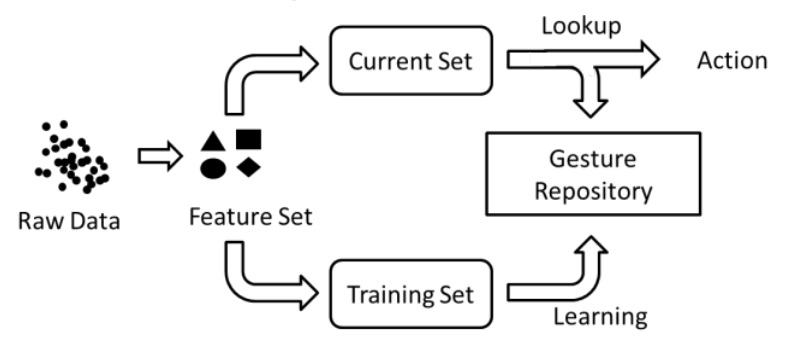
\includegraphics[width=0.7\textwidth]{images/gesture_by_example}
\caption{Principle components of a learning by example recognition framework \cite{braun2013capacitive}}
\label{fig:gesture_by_example}
\end{figure}

Initially a static gesture recognition method was implemented that used a series of five subsequent locations and simple heuristics to determine a small number of gestures. However, this limits the potential gesture set and is difficult to extend. Thus, a generic gesture recognition module was created, based on learning by example \cite{braun2013capacitive}. The general functionality of a gesture recognition framework based on learning by example is shown in Figure \ref{fig:gesture_by_example}. A feature set is extracted from incoming raw data. Collections of these are distinguished into training sets that are used to associate certain features to given gestures. After a learning process the current feature sets that are acquired on-the-fly, are tested against the training sets in a repository. These look-ups can lead to successful gesture recognition and association to certain actions. This association method is also called classification. There are numerous approaches, e.g. neural networks (NN) or support vector machines (SVM).

\subsubsection{Large-area location tracking}
There are several systems that use capacitive proximity sensing to track the location of one or more persons in an environment. A common challenge in large areas is achieving a suitable coverage with electrodes at all positions. Lauterbach et al. overcome this problem in their SensFloor system by integrating sensors and electrodes in an underlay that can be placed below the upper layer of the floor \cite{lauterbach2009}. TileTrack, the system developed by Valtonen et al. requires large emitter electrodes under the floor and receivers placed in the walls \cite{Valtonen2009a}. This limitation was reduced in a later iteration where they integrated receivers into different pieces of furniture.

While SensFloor allows to cover large areas by having the sensing electrodes near all surface areas, a limitation is the maintenance. If a sensor breaks below the floor covering it is difficult to replace. TileTrack in its initial installation requires proximity to walls, or later to specific pieces of furniture that are in the environment. This is difficult to guarantee in many instances and requires an initial calibration of the environment, according to placement of the furniture.

\begin{figure}[h]
\centering
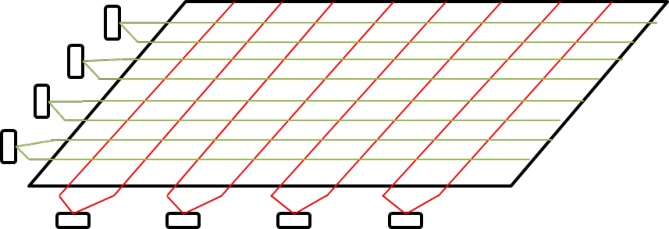
\includegraphics[width=0.8\textwidth]{images/capfloor_concept}
\caption{Wire electrode grid below floor cover attached to sensors on the border}
\label{fig:capfloor_concept}
\end{figure}

I proposed a system based on a rectangular grid of long wire electrodes that are placed below the top floor cover. The sensors are attached at the edge of the area, e.g. in skirting boards \cite{Braun2012CapFloor}. As the system is based on loading mode, there is no need for dedicated receivers, but instead it relies solely on the electrodes below the floor. The system is akin to a larger variety of projected capacitive touch screens that are partially also using grid layouts. However, those typically rely on shunt mode measurements \cite{BarrettScreen}. 

\begin{figure}[h]
\centering
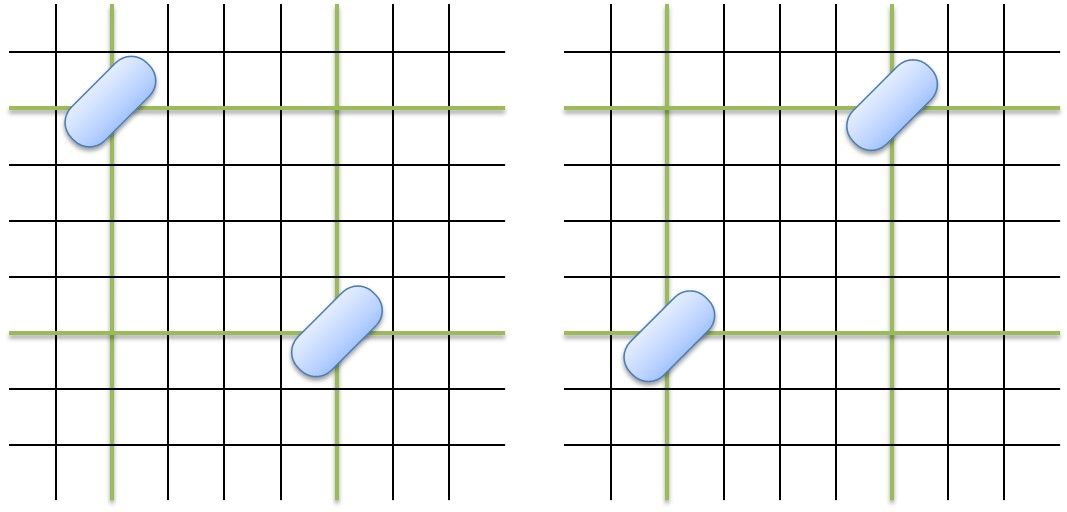
\includegraphics[width=0.8\textwidth]{images/capfloor_ghosting}
\caption{Two potential person locations resulting in same sensor readings (green indicates active electrodes}
\label{fig:capfloor_ghosting}
\end{figure}

Using long, straight wire electrodes has different effects on the measurement. One effect of this is the limited detection distance that is not comparable to large plate electrodes. Particularly if thick floor covers are used, the grid has to be fairly dense. Another effect is the sensitivity towards noise and influence from outside electric fields. Therefore, the system requires preprocessing to reduce the noise and achieve a more robust high-level data processing. In order to localize persons, the system uses an adapted weighted average algorithm, similar to the variety presented for the gesture recognition in the previous section. Each electrode is considered to only have a single coordinate in either $x$ or $y$ direction, allowing to easily calculate the center-of-gravity. However, it can occur that only two electrodes are active at a certain point in time, while two persons are present and too far away from any other electrode to be detected. In these cases there is a certain ambiguity as each $(x,y)$ value combination can result in two potential intersection points, as shown in Figure \ref{fig:capfloor_ghosting}. To overcome this problem, it is possible to either use a mix of sending and receiving electrodes operating in shunt mode and specific measurement cycles, or analyze the time-series of previous locations to discard unlikely positions.

\begin{figure}[h]
\centering
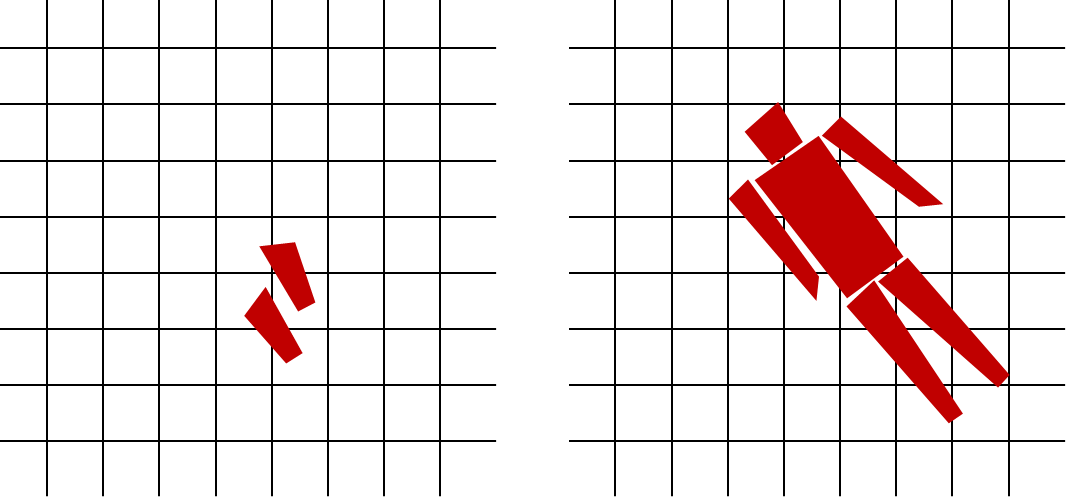
\includegraphics[width=0.8\textwidth]{images/floor_shapes}
\caption{Shapes of a standing and lying person on top of the CapFloor grid}
\label{fig:capfloor_shapes}
\end{figure}

Similar to SensFloor, the concept also supports detecting additional information about the persons present, most notably fall detection. This is based on a time-series analysis of aggregated values of the sensors that are currently detecting an object. This method is using the assumption that the overall sensor response is roughly equivalent to the shape of the object that is closest to the surface. This results in a higher capacitance of the overall system, similar to the plate capacitor model. The effect is shown in Figure \ref{fig:capfloor_shapes}. The sum $s$ of all n sensor values $r$ is the closest equivalent to the system capacitance and therefore a viable measure. If the overall value is beyond a certain threshold $v_l$, we can consider a lying person $p_l$.
\begin{align}
s&=\sum^n_{i=0}{r_i} & p_l&=\left\{ \begin{array}{c}
1,\ \ \ s\ge v_l \\ 
0,\ \ \ s<v_l \end{array}
\right.
\end{align}
In order to increase the robustness this threshold has to be exceeded for a certain amount of time $t_m$. In consequence a fall $f$ is detected if the following equation is 1.
\begin{equation}
f=\prod^{t_m}_{j=0}{p_{l,t_j}}
\end{equation}

\subsection{Model-driven fitting methods}
\subsubsection{Single-body models}
\begin{minipage}{\linewidth}
\centering
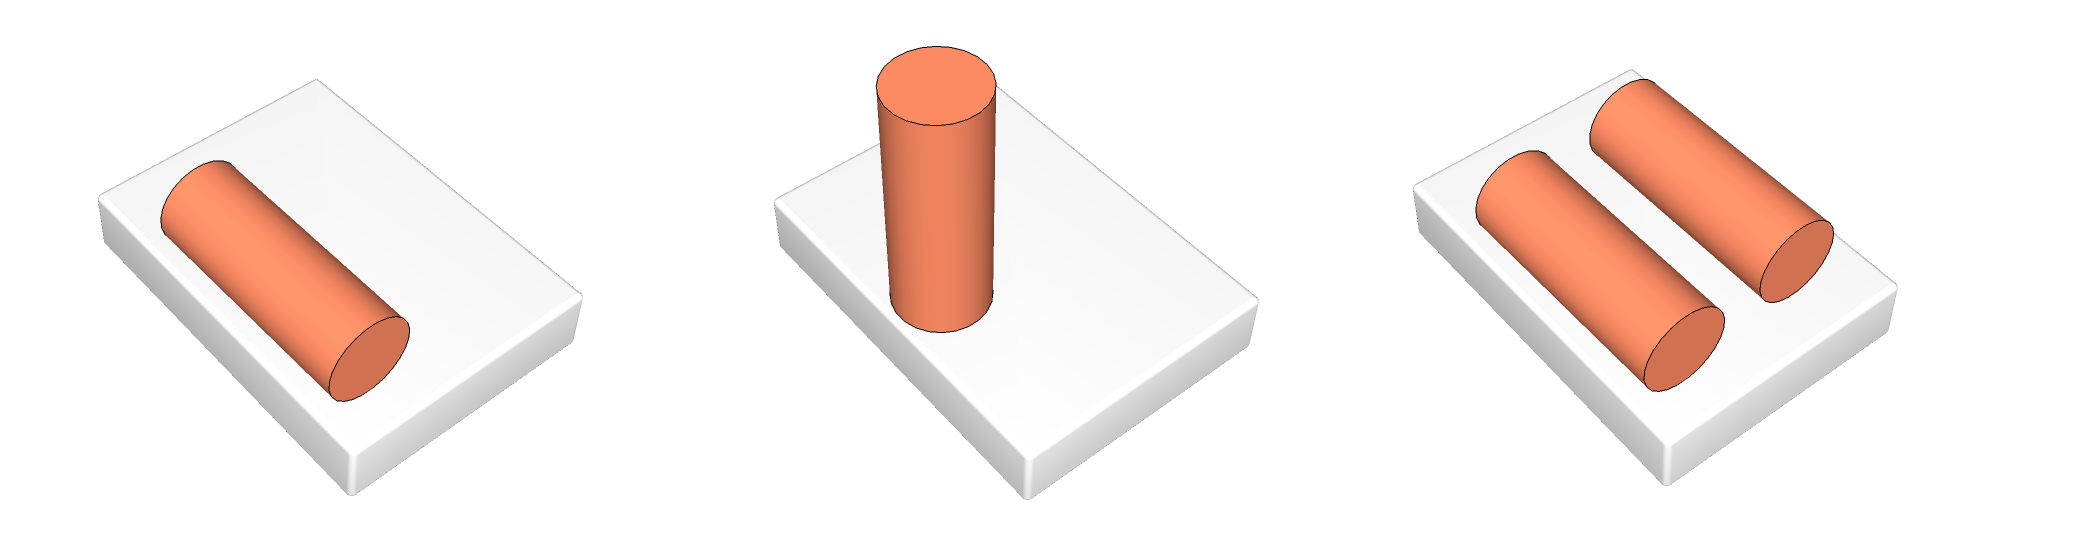
\includegraphics[width=0.8\textwidth]{images/prot_model_bed}
\captionof{figure}{Simplified human body model and various poses on mattress}
\label{fig:prot_model_bed}
\end{minipage}	

To identify occupation and positioning we use a very simple model for estimating the effect of a human body on the sensor values. As mentioned earlier the sensors act on both presence and pressure applied. We model the human body as an approximately cylinder shaped object that is on the mattress either lying or sitting, either one or two objects, a few potential poses shown in Figure \ref{fig:prot_model_bed}. We assume that the sensors are analyzing the pressure distribution on the mattress, a sitting person will cause a high pressure on a small region, a lying person a moderate pressure on a larger region. Determining the position and orientation of this cylinder from a limited amount of sensor readings can be postulated as an inverse problem. If we assume a constant density of the cylinder the idealized pressure distribution is uniform as shown in Figure \ref{fig:prot_model_pressure}.
\begin{minipage}{\linewidth}
\centering
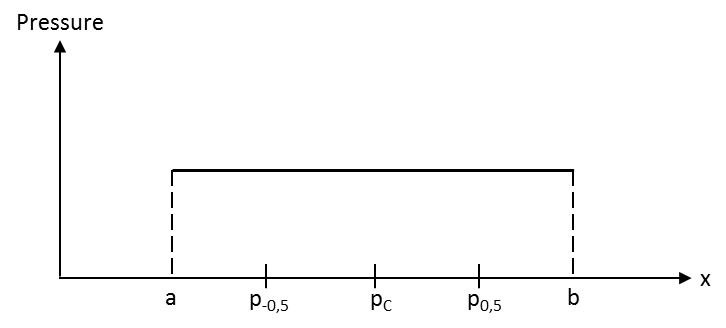
\includegraphics[width=0.6\textwidth]{images/prot_model_pressure}
\captionof{figure}{Pressure distribution of a uniform cylinder}
\label{fig:prot_model_pressure}
\end{minipage}

We further simplify the system by using two distinct values of the pressure distribution. $p_c$ is the center of pressure, $p_{-0.5}$ and $p_{0.5}$ the points enclosing half of the pressure distribution. Using the calculations of a regular uniform, continuous distribution we get the following equations:

\begin{align}
p_c&=\frac{a+b}{2} & \sigma&=\sqrt{\frac{(b-a)^2}{12}}
\end{align}
\begin{align}
p_{-0.5}&=p_c-\sigma &	p_{0.5}&=p_C+\sigma
\end{align}

The raw data from the sensor is considered as random, uniform sampling, a discretization of the continuous distribution. We calculate the center of pressure and the standard deviation of using the geometric meta-information, the position of the sensor $\overrightarrow{x}$.
\begin{equation}
p_c=\frac{\sum_{i=1}^n{v_i\overrightarrow{x}}}{\sum_{i=1}^n{v_i\overrightarrow{x}}}
\end{equation}
\begin{equation}
\sigma=\sqrt{\frac{1}{n}(\sum_{i=1}^n{\overrightarrow{x}^2}-\frac{1}{n}(\sum_{i=1}^n{\overrightarrow{x}})^2}
\end{equation}

Using this model we have determined a set of potential poses that cover the most common situations. We distinguish between potential poses for one and two occupants. One person may sit at a certain location or lie on the bed in various angles. It is assumed that the head is always at the upper part of the bed. Two persons may either both sit, both lie down, or one is sitting and one lying. 
The limitations of this model concerning the actual system are the non-uniform pressure propagation throughout the mattress, as well as the non-linear sensor response on different pressure levels. Therefor we do not expect the deviations to strictly adhere to the theoretical model but instead use configurable thresholds that allow for increased robustness in exchange for precision.

\begin{figure}[h]
\centering
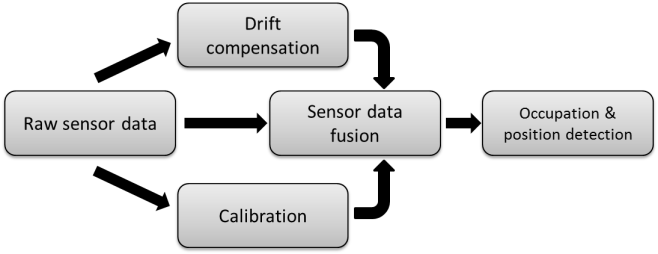
\includegraphics[width=0.7\textwidth]{images/smartbed_proc}
\caption{Data processing components \cite{braun2012context}}
\label{fig:smartbed_proc}
\end{figure}
The different components of the Smart Bed data processing are shown in Figure \ref{fig:smartbed_proc}. Raw sensor data is distributed to three different modules, the calibration which is determining the initial parameters for the sensor data fusion, the drift compensation that alters those parameters according to long term trends and finally the sensor data fusion module that processes the data and does feed it to the occupation \& position detection. Calibration and drift compensation follow the previously presented model \cite{braun2012context}. 
\begin{figure}[h]
\centering
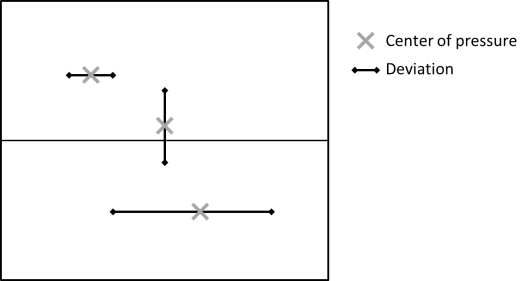
\includegraphics[width=0.7\textwidth]{images/smartbed_cog}
\caption{Calculating centers of pressures and deviation \cite{braun2012context}}
\label{fig:smartbed_cog}
\end{figure}
Occupation and position detection is performed by dividing the two person bed into left and right and individually calculating for each side the total sensor values, assumed center of pressure using weighted average and the standard deviation (Figure \ref{fig:smartbed_cog}). The same calculation is done between the two sides to distinguish where is activity or if one person is lying diagonally.
Using these six intermediate values we can now map various poses. If all activity is on one side and the horizontal deviation is low, we can assume that one person is sitting. We can additionally use the intermediate values to calculate more information, e.g. the exact location a person is sitting at. 
The data processing for the sleep phase recognition is based on detecting the sensor data variations in order to analyze movement. Discriminating between sleep phases using movement is a common approach that has been used in the past \cite{salmi86}. Using a sparse set of sensors it is possible to detect movement by comparing subsequent sensor readings and associate it to different sleep phases using different activity profiles. The system is based on the same prototype as the posture recognition system \cite{Djakow2013movibed}.
\subsubsection{Multi-body models}
\begin{figure}[h]
\centering
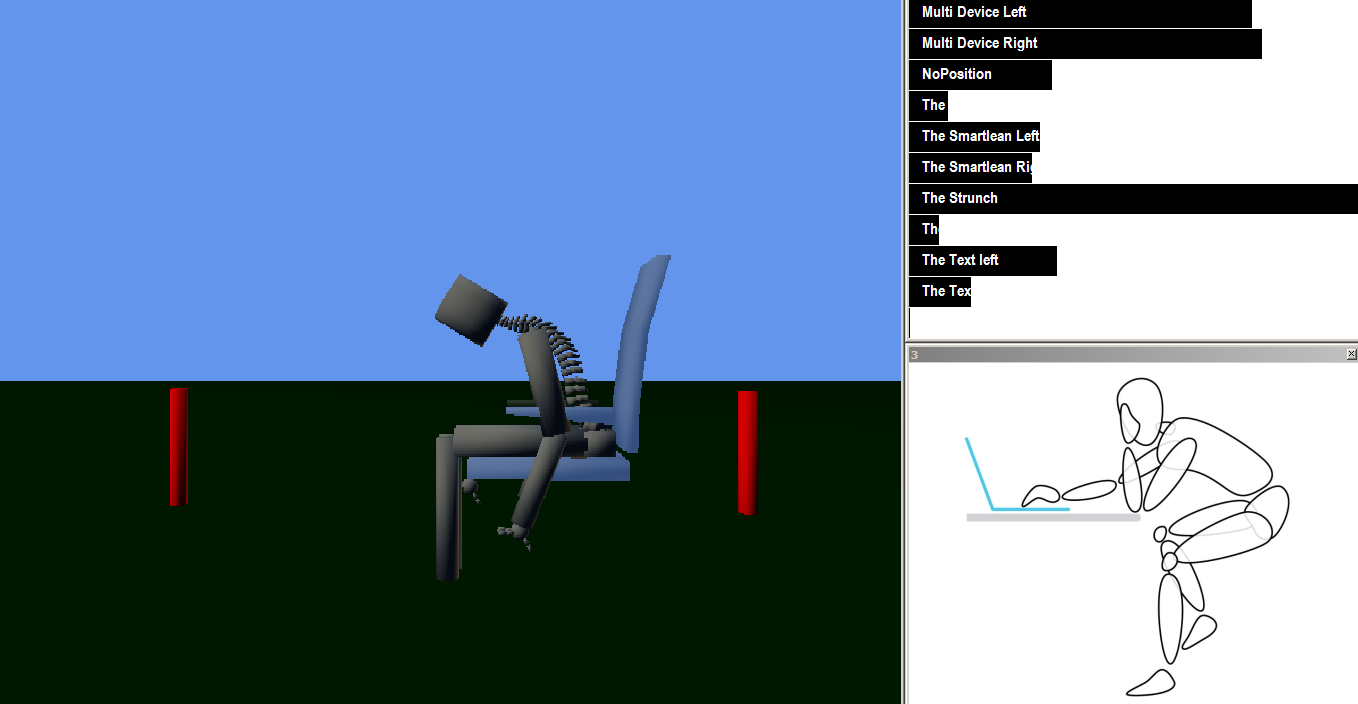
\includegraphics[width=0.7\textwidth]{images/smartchair_software}
\caption{Screenshot of the Capacitive Chair application showing the fitted 3D model on the left, posture detection on the upper right and the recognized posture on the lower right}
\label{fig:smartchair_software}
\end{figure}
In Figure \ref{fig:smartchair_software} we can see a screenshot of the Capacitive Chair debug application. On the left side we see a 3D model that is fitted to a chair model according to the current sensor values, in the middle the results of the machine learning module and the recognized posture and on the right side the currently running breathing rate detection as both Fourier analysis and signal deviation analysis.
All processing methods work on filtered and normalized sensor data. The difference in shape, material and size of the electrodes necessitates slight adaptations to noise filtering and data processing. As an example only the conductive thread backrest electrode is used in the breathing rate detection. 
The 3D model is using a simplified human joint model comprised of 13 connected components. Based on the current sensor readings, single parts or groups of components are fitted to the virtual chair. The process is a mix of posture mapping as found in the smart bed and modification of the dynamic links between the single components \cite{Braun2013ChairAid}.
\begin{figure}[h]
\centering
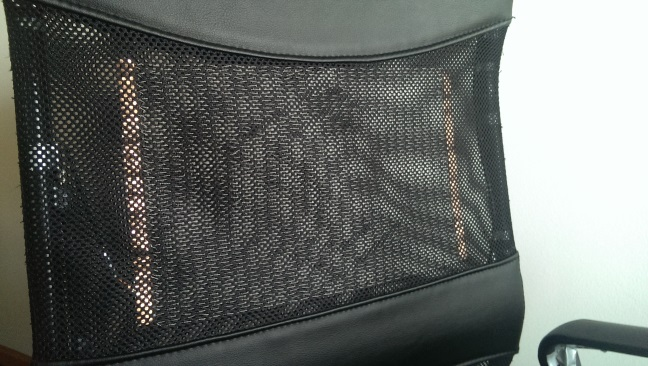
\includegraphics[width=0.7\textwidth]{images/smartchair_thread}
\caption{Screenshot of the Capacitive Chair application showing the fitted 3D model on the left, posture detection on the upper right and the recognized posture on the lower right}
\label{fig:smartchair_thread}
\end{figure}
We use a simple RBF neural network and training data collected by two different persons to match the input from eight sensors to nine potential output postures that are associated to different working situations. An early observation is that certain postures are difficult to distinguish given the limited number of sensors and the similarity of the postures on the rigid chair. Either a higher number of sensors or a more versatile chair could be used that allows gathering additional information required to distinguish the different poses more reliably. 

The breathing rate detection is operating on a single electrode that is integrated into a mesh on the backrest using conductive thread. The setup is shown in Figure \ref{fig:smartchair_thread}. Consequently the surface of the electrode is large and able to pick up the chest movement. Two different methods of data processing are used and fused to get the final breathing rate. Using a fast Fourier transformation the signal is transformed into the frequency space. We are looking for significant signal portions in frequency areas that can be associated to breathing, between $0.2Hz$ and $10Hz$. The second method is to look for zero-crossings of the sensor signal through an adaptive baseline. If a person is breathing in the sensor value will decrease resulting in the signal dropping below the long-term average, and rise above when the person is breathing out. Accordingly the breathing rate can be calculated by counting the zero-crossings.
\subsection{Heterogeneous sensor systems}
\subsubsection{Heterogeneous capacitive arrays}
\begin{figure}[h]
\centering
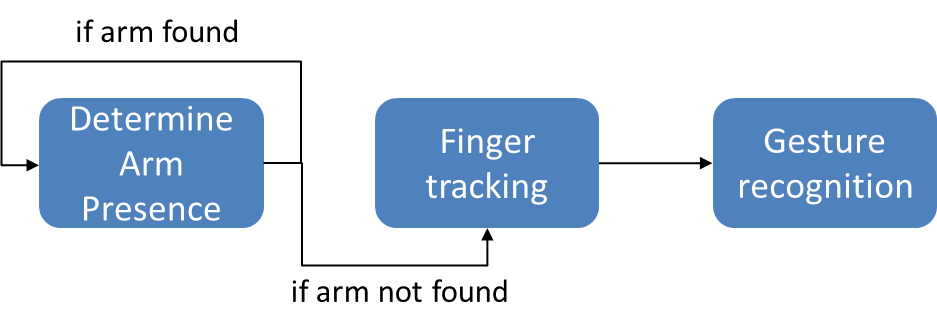
\includegraphics[width=0.4\textwidth]{images/armrest_dataproc}
\caption{Data processing pipeline of Active Armrest}
\label{fig:armrest_dataproc}
\end{figure}
%Figure 25 Data processing pipeline of Active Armrest
As we already mentioned, the Active Armrest electrodes are put into two groups. The data processing for both groups is distinctly different. In order to detect the presence of the arm using the two-electrode group a simple threshold on the accumulated values is used. The six sensor array in the front (touch area) is using the presented weighted average method to calculate finger positions. Additionally a threshold is used to distinguish one and two fingers. Overall there is a data processing pipeline as shown in Figure \ref{fig:armrest_proto}. The finger tracking and gesture recognition will be inactive until it is ensured that no arm is present. 

\subsubsection{Heterogeneous sensor fusion}
\begin{figure}[h]
\centering
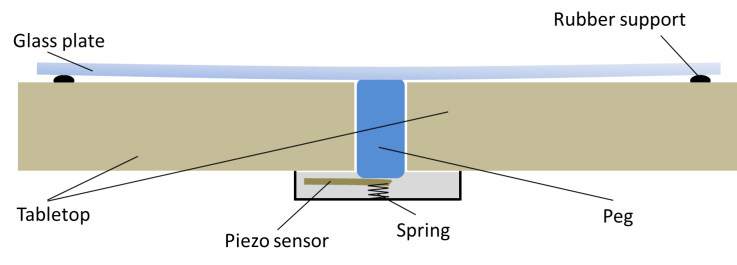
\includegraphics[width=0.7\textwidth]{images/captap_peg}
\caption{Suspended peg knock detection system for CapTap \cite{Braun2013ChairAid}}
\label{fig:captap_peg}
\end{figure}
%Figure 34 Suspended peg knock detection system for CapTap [80]
The hand location of the CapTap is similar to the methods presented for the MagicBox. We add the additional component of knock detection to provide selection events when touching the surface. Figure \ref{fig:captap_sketch} shows a sketch of the knock detection system. The table has a glass plate that is suspended on some rubber supports. In the center of the table we attach a small peg (enlarged in sketch) that creates a connection between the glass plate and a piezo sensor. If the glass plate starts vibrating from a touch we can measure this using the piezo sensor \cite{Braun2013ChairAid}. If a notable vibration is measured we are collecting the next 50 samples, resulting in a window of 250 milliseconds. To distinguish single and double knocks we calculate the weighted average within this window to get a measure for the distribution of sensor values within. If the average is closer to the beginning of the window the resulting event should be a single knock, and a double if the average is closer to the end of the window.
Hand localization and knock detection are working independently and are combined later in the software. It is reasonable to combine this, e.g. to ignore knock events that are occurring without a hand present. They may be indicative of a person doing a strong step close to the table.

\subsection{Image-based processing}
Their ability to detect changes in the electric field over a distance has led to capacitive proximity being regarded as similar to cameras. Smith et al. consequently called their approach electric field imaging, as particularly shunt mode measurements and their constrained electric fields allow applying certain image processing methods, e.g. tomography \cite{Smith1999a}. They were critical of using similar methods for shunt mode, noting the following statement.
\begin{quote}
Loading mode measurements can be likened
to images formed without a lens, since only one "end" of
each field line is constrained by the measurement. \cite{smith1998electric}
\end{quote}
Nonetheless, loading mode has certain advantages, particularly if all electrodes are in a single plane and we would like to have a higher sensitivity at a distance from the plane it is advantageous if there is no receiving potential nearby. One example for this planar electrode setup is large area gesture interaction devices, e.g. a table that is able to track the position of arms and hands in three dimensions. There is a plethora of image-based object detection and tracking algorithms that can be also used for capacitive proximity sensor data processing. There is a short process that I propose to realize this arm and hand tracking that includes some general steps that can be used to identify a variety of objects. The process is distinguished into four distinct steps:
\begin{itemize}
\item Creating a grayscale image from the acquired sensor data
\item Apply a feature-preserving image upscaling method
\item Find the contours of the present objects according to pixel values
\item Analyze the image moments of the contour areas and fit human arms
\end{itemize} 

\begin{figure}[h]
\centering

\includegraphics[width=0.5\textwidth]{images/proc_im_pixels}
\caption{Pixel array mapped from sensor values}
\label{fig:proc_im_pixels}
\end{figure}

The most challenging aspect of the first step is the low resolution of a reconstructed image. In order to achieve a mid-range distance resolution that allows detecting objects within 30 or 40 cm it is necessary to use electrodes that are sufficiently large. Thus, an example device uses an array of 6x4 sensor electrodes, resulting in an image of only 24 pixels. Typically the sensor values are an integer value in a range between 0 and 15000. Accordingly we can create a single-channel image with a channel depth of two bytes. In our case we use a linear mapping of sensor values to pixel intensities. An exemplary result image of this mapping is shown in \ref{fig:proc_im_pixels} (with enlarged pixels). In this format it is difficult to gather information about the exact position of the arms and thus we need to apply further processing before finding the contours and fitting arm objects.
\begin{figure}[h]
\centering
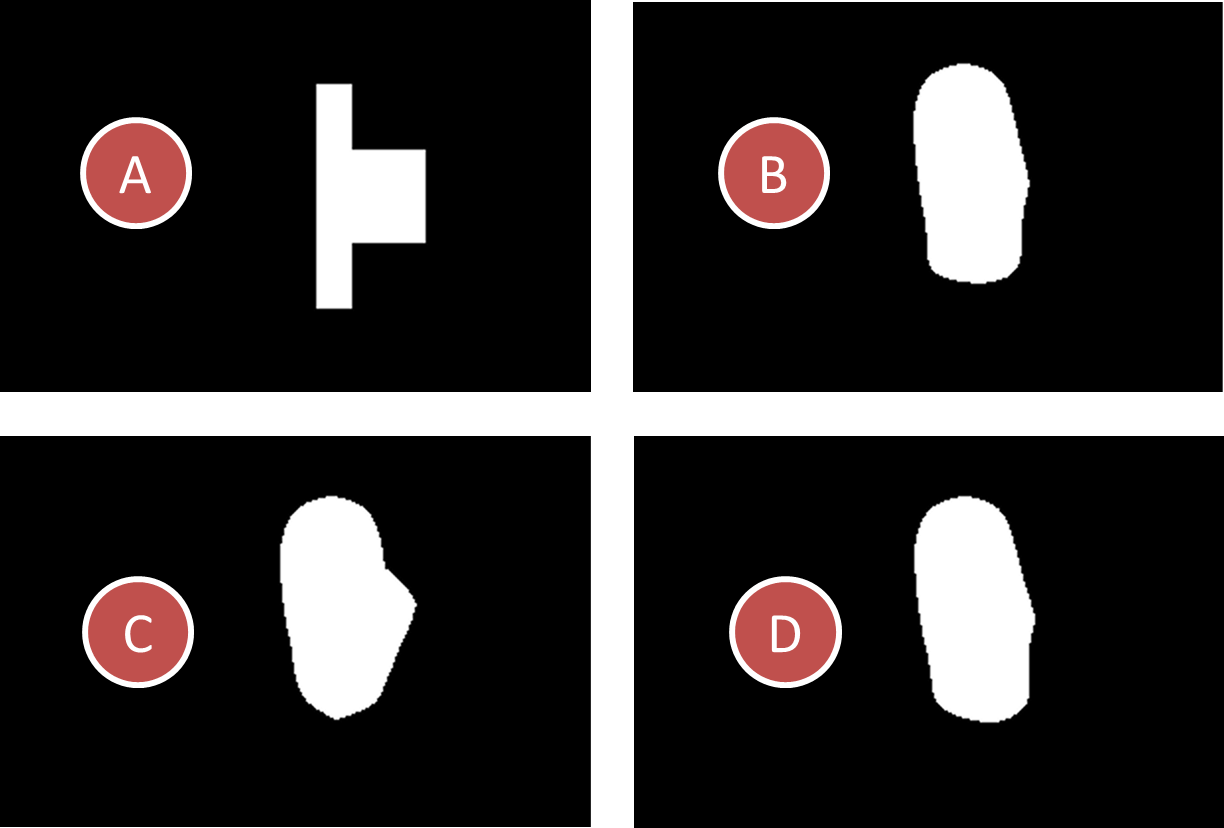
\includegraphics[width=0.9\textwidth]{images/proc_im_interpol}
\caption{Effect of different upscaling methods on shape, (A) nearest neighbor, (B) bicubic, (C) bilinear, (D) Lanczos4 - shown as thresholded binary images (pixel intensity > 30)}
\label{fig:proc_im_interpol}
\end{figure}

\subsubsection{Acquire and optimize contours}
In order to get the relevant contours of objects in the interaction area we have to apply some further processing. The first step is to enlarge the image using a feature-preserving scaling method. As all sensors are prone to environmental noise we apply some thresholding based on the pixel intensities before looking for contours. The result is an enlarged binary image of black and white pixels. We have tested four different image scaling methods, nearest neighbor, bilinear interpolation, bicubic interpolation and Lanczos interpolation. Exemplary results are shown in \ref{fig:proc_im_interpol}. The Lanczos interpolation showed the best results but is most processing intensive. However, since we are dealing with small images it is reasonable for CapTap. The contours are calculated based on those binary images, defined as the borders between black and white regions. For further processing we are looking into the distribution and the intensities of the pixels within the specified region.
\begin{figure}[h]
\centering
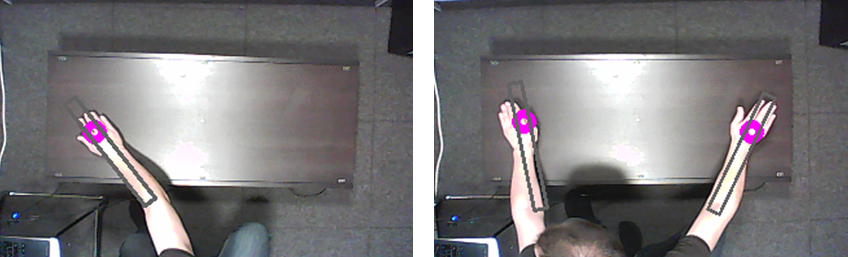
\includegraphics[width=0.9\textwidth]{images/proc_im_arms}
\caption{Overhead camera picture of the scene overlaid with live arm and palm reconstruction for one arm (left) and two arms (right)}
\label{fig:proc_im_arms}
\end{figure}

\subsubsection{Palm and arm fitting}
The last step of identifying and tracking the arms is to fit the position and orientation of the palms and arm into the acquired object contours. For this task we are analyzing the image moments within the contours. These are certain particular weighted averages of pixel intensities, or a function thereof \cite{hu1962visual}. They can be calculated using the following equation, whereas $j$ and $i$ define the order and $I(x,y)$ is the pixel intensity at a given position. We can use this to calculate the center point $(\overline{x},\overline{y})$, leading to the central moments $mu_ji$ that are required to determine the orientation of the contour as angle $\gamma$.
%m_ji=∑_(x,y)▒〖I(x,y) x^j y^i  〗,x ̅=m_10/m_00 ,y ̅=m_01/m_00 
%〖mu〗_ji=∑_(x,y)▒〖I(x,y) (x-x ̅ )^j (y-y ̅ )^i  〗
% γ=0.5∙arctan (2∙〖mu〗_11)/(〖mu〗_20-〖mu〗_02 )
\begin{equation}
m_ji=\sum_{(x,y)}{I(x,y)x^jy^i}
\end{equation}
\begin{equation}
\overline{x}=\frac{m_10}{m_00}, \overline{y}=\frac{m_01}{m_00}
\end{equation}
\begin{equation}
mu_{ji}=\sum_{(x,y)}{I(x,y)(x-\overline{x})^j(y-\overline{y})^i}
\end{equation}
\begin{equation}
\gamma=0.5\cdot arctan\frac{2\cdot{mu_{11}}}{mu_{20}-mu_{02}}
\end{equation}
 
We use the center point and orientation to calculate the estimated position of the palm of the hands. These points are the basis for the subsequent gesture recognition. Additionally, we are using separate Kalman filters for smoothing the different palm positions and arm orientation. The resulting arm reconstruction and the actual arm position in a photo are shown in \ref{fig:proc_im_arms}. We installed a simple webcam above the table and registered the table position to the camera image. 

The arm reconstruction so far is mostly used to determine the arm position. Another potential use of the arm orientation is to improve the merging of two hands. While the system can't distinguish from a single sensor if one hand is close or two hands are further away, we can use the presence of two arms to identify the overall number of objects in the detection range. 
\subsubsection{Intensity-based elevation estimate}
A distinct challenge of the capacitive hand tracking is the considerable directional difference in available resolution. While we can use the presented image analysis to track the planar position of the arms over the whole table area of 80cm width and 50cm depth, estimating the elevation of the arm above the table is restricted by the proximity range of the single sensor. Typically the achievable range maxes out at around 35cm, depending on environmental conditions. In a plate capacitor system the distance $d$ is proportional according to size of the plates $A$ and resulting capacitance $C$. Due to the linear mapping of sensor capacitance measurements to pixel intensities $I$ we can use the image moment within a contour $S$ as estimate of the actual capacitance, and calculate the elevation $e$ according to the following equations:

\begin{align}
d&\propto{\tfrac{C}{A}} & S&\propto{\tfrac{m_{00}}{\int{S}}}
\end{align}

The same thresholds discussed in the contour retrieval phase apply to this step, thus leading to discarding objects at a larger distance that are difficult to detect. Starting from this threshold we normalize the resulting elevation according to a maximum threshold for m00 that denotes a very close object (such as touch). The actual touch recognition is performed using acoustic methods. 
As previously explained the sensors are prone to environmental influences, thus this just allows to get an estimate of the actual elevation and no absolute distance value. Therefore, the interaction should not be designed to require a highly precise discrimination of different elevation values, but instead use more of a 2.5D paradigm. Our take on this will be presented in the application section.
\subsection{Physiological signals in frequency- and time-domain}
\subsubsection{Respiratory rate}
\subsubsection{Sleep phase recognition}
The most reliable way to track sleep phases is by using an electroencephalography (EEG); that is measuring the electrical activity of the brain by placing electrodes on the scalp. Various different types of neural oscillations can be distinguished - the most important for sleep phase detection are alpha waves, theta waves, delta waves and sleep spindles. The American Academy of Sleep Medicine (AASM) distinguishes three different phases of non-rapid eye movement sleep (NREM) and REM phase [11]. 
\begin{itemize}
\item Stage 1 - occurs mostly in the beginning of sleep. It has slow eye movement, alpha waves disappear and the theta wave appears. 
\item Stage 2 - dreaming is very rare and no eye movement occurs. The sleeper is quite easily awakened. EEG recordings have a tendency for characteristic "sleep spindles"
\item Stage 3 - was previously divided into stages 3 and 4. It is slow-wave sleep (SWS) or deep sleep. Stage 3 used to be the transition between stages 2 and 4 where delta waves began to occur, while delta waves are dominant in stage 4. 
\item REM sleep - is a phase of sleep characterized by random and rapid movement of the eyes. It is considered the lightest phase of sleep and occurs all through the night but gets longer close to morning.
\end{itemize}

\begin{minipage}{\linewidth}
\centering
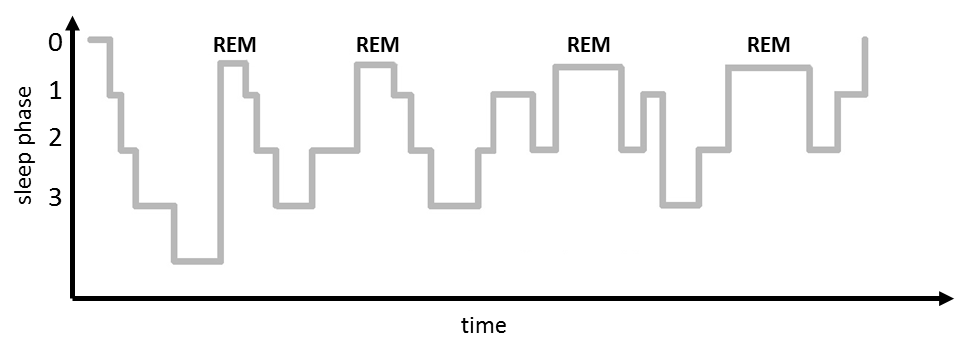
\includegraphics[width=0.6\textwidth]{images/proc_phys_sleepphase}
\captionof{figure}{Example of human sleep phases throughout the night}
\label{fig:proc_phys_sleepphase}
\end{minipage}

A typical distribution of sleep phases throughout the night is shown in Figure \ref{fig:proc_phys_sleepphase}. It can be easily seen that the sleep is distributed into different cycles, whereas the sleeping person is moving through the different sleep phases until having a REM phase and then going back to deep sleep. If the only available data is body movements it is becoming more difficult to reliably determine the sleep phase. Studies have shown that the magnitude of movement is typically associated to the follow-ing phases in decreasing order: wake, stage 1, REM, stage 2, stage 3 [12]. Another method is distinguishing between awake phase, active sleep and quite sleep and takes into account the order of those phases. This information allows to correlate the actual sleep phases with good certainty [13]. We have chosen this method for our system.

Capacitive proximity sensors enable us to detect the presence of suitable object and their relative proximity to the electrode. Consequently a moving object will cause a change of sensor values. If we aggregate these data deviations from an array of sensors we get a reliable measure of objects moving above the electrodes. In the case of MoviBed we can assume that there is a limited number of persons moving on top of the sensors and thus it is possible to associate the sensor values to movement. In the following we will present a suitable method to achieve a reliable detection of the movements of a sleeping person. We are following a similar approach as Salmi and Leinonen [13].
At any given time t a set of the latest values of all n sensors can be stored as a tuple in the following form: 
\begin{equation}
\overrightarrow{s_t}=\begin{pmatrix}
s_{1_t}\\ 
s_{2_t}\\ 
\vdots \\ 
s_{n_t}
\end{pmatrix}
\end{equation} 

%(s_t ) ⃗=(■(s_(1_t )@s_(2_t )@■(⋮@s_(n_t ) )))
As capacitive proximity sensors are particularly susceptible to external influences, such as temperature, humidity and other electric fields it is necessary to apply filtering on the sensor values. A suitable candidate is a median filter - a low-pass filter method that selects the median object of a sorted set of values, thus discarding outliers and strongly deviating values. This is particularly suited if transmission errors may occur.
If a person is moving on the bed the value of all sensors in detection distance of the moved body parts will change accordingly, the most relevant example in our case being a person moving in its sleep. We can generate a measure of movement intensity by comparing the values at time t with those at time t-1 resulting in:
\begin{equation}
\overrightarrow{d_t}=\left | \overrightarrow{s_t}-\overrightarrow{s_{t-1}} \right | = \begin{pmatrix}
\left | s_{1_t}-s_{1_{t-1}} \right |\\ 
\left | s_{2_t}-s_{2_{t-1}} \right |\\ 
\vdots \\ 
\left | s_{n_t}-s_{n_{t-1}} \right |
\end{pmatrix}
\end{equation}
%(d_t ) ⃗=|(s_t ) ⃗-(s_(t-1) ) ⃗ |=(■(|s_(1_t )-s_(1_(t-1) ) |@|s_(2_t )-s_(2_(t-1) ) |@■(⋮@|s_(n_t )-s_(n_(t-1) ) | )))
In subsequent calculations we will use $\overrightarrow{d_t}$ as combined measurement. For distinguishing between wake, active sleep and quiet sleep we are solely interest in the most intense movement. Thus we are testing for the largest value over a set of $m$ samples, generating the value $b_t$.
\begin{equation}
b_t=max(\overrightarrow{d_t1, d_t2, \hdots, d_tm}
\end{equation}
%b_t=max⁡((d_t1 ) ⃗,(d_t2 ) ⃗,…,(d_tm ) ⃗)
The value $b_t$ is affected by changes in the speed of movement. Therefor as a final step we generate a centered average value of order $2q-1$:
\begin{equation}
\overline{b_t}=\frac{1}{2q-1}\sum_{i=-1}^q{b_{t-i}}
\end{equation}
%(b_t ) ̅=1/(2q-1) ∑_(i=-q)^q▒b_(t-i) 
The resulting value $\overline{b_t}$ allows us to quantify the intensity of movements over a given period. In order to extract an actual body movement from this value we have to quantify a threshold $s(t)$ that is determined by the average of $q$ previous values of $\overline{b_t}$ multiplied with a factor $f$ that has to be evaluated individually for each configuration of bed and sensors. This threshold $s(t)$ allows us to identify a movement $m$ at any time $t$. This behavior is denoted in the following equations:
\begin{equation}
s(t)=\left ( \frac{1}{q}\sum_{i=1}^{q+1}{\overline{b_{t-1}}} \right )\cdot f
\end{equation}
\begin{equation}
m_t=\left\{\begin{matrix}
1,if \; \overline{b_t}> s(t)>\overline{b_{{t-1}}}\\ 
0,else
\end{matrix}\right.
\end{equation}

As previously mentioned it is difficult to determine sleep phases solely by monitoring the movement. Instead following the example of Salmi and Leinonen and distinguish three phases - wake, active sleep and quiet sleep [13]. These are determined by dividing the sleep time into $a$ three-minute epochs $e_{i_a}$ and qualify these as active or quiet by counting the number of movements occurring in those intervals and comparing it to the average amount of movements in all epochs $\overline{e_a}$ determined by the following equations:
\begin{align}
e_{i_a}&=\sum_{e_{i_Start}}^{e_{i_End}}{m_i} & \overline{e_a}&=\frac{1}{n}\sum_{i=0}^n{e_{i_a}}
\end{align}
%e_(i_a )=∑_(e_(i_Start ))^(e_(i_End ))▒m_i    ,    (e_a ) ̅=1/n ∑_(i=0)^n▒e_(i_a ) 

In consequence we determine the status of any epoch with this final equation:
\begin{equation}
e_{i_a}=\left\{\begin{matrix}
active,if \; e_{i_a}>\overline{e_a}\\ 
quiet,if \; e_{i_a}\leq \overline{e_a}
\end{matrix}\right.
\end{equation}
%e_(i_a )={█(active,if e_(i_a )>(e_a ) ̅  @quiet,ife_(i_a )≤(e_a ) ̅ )┤
These active and quiet periods can be semi-autonomously interpreted by humans in order to determine the actual sleep phases. For example initial activity for 20 to 40 minutes followed by a quiet period can be attributed to a person falling asleep. Following quiet phases are a good indicator for deep sleep phases.
 


